
\part{Praxisteil}

Versuchsaufbau:

Testplattform: pludoni Server eq4
Prozessor: Intel® Core™ i7-920
Arbeitsspeicher: 8 GB DDR3 RAM
Festplatten: 2 x 750 GB SATA-II HDD (Software-RAID 1)
Netzwerkverbindung: 100Mbit

Livesystem: pludoni Server 
Prozessor: Intel® Core™2 Quad CPU Q6600 @ 2.4 Ghz
Arbeitsspeicher: 4 GB DDR3 RAM
Festplatten: 2 x 750 GB SATA-II HDD (Software-RAID 1) %TODO aktualisieren
Netzwerkverbindung: 100Mbit

Testclient: Virtualbox
Firefox 5

Testobjekt:
Itsax Startseite


Ausgangszustand:
Sreeram Ramachandran ein Software Engineer bei der Firma Google hat eine Analyse über 4.2 Milliarden Seiten veröffentlicht. Diese ist im Rahmen der Initiative ``Let's make the web faster'' entstanden und zeigt häufige Fehlerquellen und ungenutztes Potential auf. Die durchschnittliche Webseite hat laut Ramachandran 320 KB Größe, 44 verschiedene Ressourcen und es werden nur 66\% der komprimierbaren Inhalte tatsächlich komprimiert.
Itsax.de hat 106 Ressourcen und 444 KB an Daten. Schon anhand dieser zwei Zahlen lässt sich eine vergleichsweise schwache Leistung vorhersehen. Besonders die Anzahl an verschiedenen Ressourcen deutet auf Missstände hin, da Parallelisierung von Zugriffen nur bis zu einem bestimmten Grad möglich ist. Die Time to First Byte(TtFB) von 674ms bezeichnet die Zeit die vergeht bis der Webbrowser die ersten Daten empfängt, dass bedeutet aber noch nicht das der Nutzer schon Inhalte präsentiert bekommt. Die Inhalte werden erst angezeigt nachdem die Time to Start Render(TtSR) vergangen ist, der Nutzer muss demnach ungefähr zwei Sekunden warten bis die Webseite im Browser anfängt sich aufzubauen. Die Load Time(LT) bezeichnet dann die Zeit die vergeht bis die Seite komplett dargestellt wird und der Benutzer sie ohne Einschränkungen bedienen kann. Es können  aber auch nach der LT noch Inhalte nachgeladen werden, wie zum Beispiel gestreamte Videos oder andere asynchrone Inhalte. Diese nachgeladenen Inhalte wirken sich aber nicht mehr Negativ auf die User Experience aus, solange sie im Rahmen bleiben und nicht wichtige Teile der Webseite wie zum Beispiel das Hauptmenü noch per Flash geladen werden müssen. Die Anzahl der DOM Elemente bezeichnet alle vom Browser zu verarbeitenden Objekte und ist ein Indikator für die Komplexität der Webseite, je mehr Elemente also vorhanden sind desto länger muss der Browser die Positionierung und Darstellung berechnen. Die Inhalte auf der Seite Itsax.de sind in Abbildung ? dargestellt, einmal im Bezug auf Größe und einmal aufgeschlüsselt nach der Anzahl der benötigten Requests um die Inhalte vom Server anzufordern. 

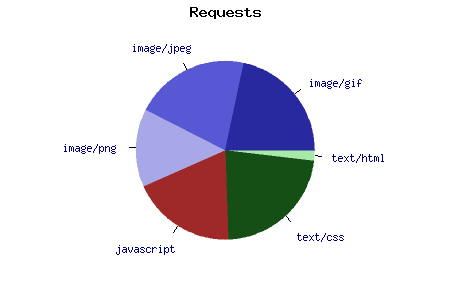
\includegraphics[scale=0.5]{material/start_request_pie.png}
\begin{tabbing}
Request \quad\= blablabla \quad\= \kill
\textbf{Typ} 	 \> \textbf{Anzahl} \\
text/css	 \>	24 	\\
image/gif	 \>	23 	\\
image/jpeg	 \>	22 	\\
javascript	 \>	20 	\\ 
image/png	 \>	15 	\\
text/html	 \>	2 	\\

\end{tabbing}

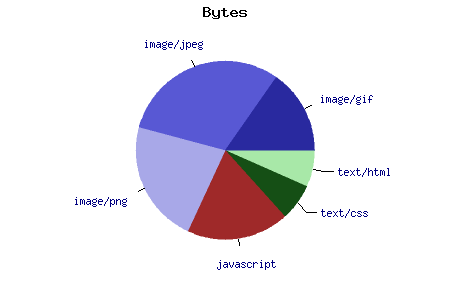
\includegraphics[scale=0.5]{material/start_byte_pie.png}

%http://code.google.com/intl/de/speed/articles/web-metrics.html

%TODO Bilder einfügen aus materials

text/css24
image/gif	22
image/jpeg	22
javascript	20
image/png	15
text/html	3

image/jpeg	142251
image/png	101428
javascript	84758
image/gif	73378
text/css	30222
text/html	29917
Ausgangssituation:
Server Software:        Apache/2.2.16
Server Hostname:        itsax.it-jobs-und-stellen.de
Server Port:            80

Document Path:          /
Document Length:        65218 bytes

Concurrency Level:      1
Time taken for tests:   18.182 seconds
Complete requests:      50

Write errors:           0
Total transferred:      3266726 bytes
HTML transferred:       3239226 bytes
Requests per second:    2.75 [\#/sec] (mean)
Time per request:       363.640 [ms] (mean)
Time per request:       363.640 [ms] (mean, across all concurrent requests)
Transfer rate:          175.46 [Kbytes/sec] received




Mit APC aktiviert:
Server Software:        Apache/2.2.16
Server Hostname:        itsax.it-jobs-und-stellen.de
Server Port:            80

Document Path:          /
Document Length:        64842 bytes

Concurrency Level:      1
Time taken for tests:   11.681 seconds
Complete requests:      50

Write errors:           0
Total transferred:      3261730 bytes
HTML transferred:       3234230 bytes
Requests per second:    4.28 [\#/sec] (mean)
Time per request:       233.620 [ms] (mean)
Time per request:       233.620 [ms] (mean, across all concurrent requests)
Transfer rate:          272.69 [Kbytes/sec] received

Mit Drupal Cache in normal Einstellung:
Server Software:        Apache/2.2.16
Server Hostname:        itsax.it-jobs-und-stellen.de
Server Port:            80

Document Path:          /
Document Length:        65005 bytes

Concurrency Level:      1
Time taken for tests:   2.082 seconds
Complete requests:      50
Failed requests:        0
Write errors:           0
Total transferred:      3276900 bytes
HTML transferred:       3250250 bytes
Requests per second:    24.02 [\#/sec] (mean)
Time per request:       41.638 [ms] (mean)
Time per request:       41.638 [ms] (mean, across all concurrent requests)
Transfer rate:          1537.09 [Kbytes/sec] received

Mit Drupal Cache in aggressiv Einstellung:



Test von Serverunabhängigen verbesserungen:
über das Analysetool von webpagetest.org
Testverfahren: 10 konsekutive Tests (maximum) der Durschnittlichste Testlauf wird betrachtet
Teststandort Frankfurt a. M.
Browser: IE9
Connection: DSL 1,5 Mbps / 50ms RTT
Only First View




Load Time: 3.728
Time to First Byte: 0.674s 	
Time to Start Render: 2.002s
\#DOM Elements: 855 	
\#Requests: 106
Bytes In: 444 KB
%http://www.webpagetest.org/result/110809_BH_198S4/


Im folgenden Abschnitt werden die eingesetzten Methoden dargestellt und ihre Auswirkungen auf die Webperformance der Seite ITsax.de dargestellt. 
JS Aggregation und Minifizierung mit dem Javascript Aggregation Modul:
Aggregation und Minifizierung sind Verfahren, die in der Webperformance Optimierung häufig eingesetzt werden. Für das Drupal 5 System gibt es fertige Module die diese Aufgabe übernehmen. Das Modul interveniert innerhalb des Drupal Kerns und ersetzt die Javascripts, die vorher direkt so ausgegeben wurden wie sie die Module lieferten, durch eine einzelne, das heisst aggregierte Version, die optional minifiziert werden kann. Diese Minifizierung wird natürlich genutzt und spart einige KB. Minifizierung wird ermöglicht durch die Nutzung von JSmin https://github.com/rgrove/jsmin-php/. JSmin ist ein Filter der unter anderem Kommentare entfernt und mehrere Leerzeichen zu einem zusammenfasst. Durch die Nutzung dieser Methode konnten 11 HTTP Abfragen und 11 KB an Datenvolumen eingespart werden.
Load Time: 3.658s
Time to First Byte: 0.595s
Time to Start Render: 1.915s
\#DOM Elements: 844 	
\#Requests: 95 %!
Bytes In: 432 KB
%http://www.webpagetest.org/result/110809_Z1_198TK/

CSS Aggregation und Komprimierung:
Analog zur Javascript Optimierung kann man auch die CSS Aggregation betrachten. Es werden durch Zusammenfassung der einzelnen CSS Dateien HTTP Abfragen eingespart. Wie man an der gesunkenen Anzahl der Requests sehen kann, wurden 21 Abfragen nur durch Zusammenfügen der einzelnen CSS Dateien zu einer einzigen eingespart. Durch die Bereinigung beziehungsweise Komprimierung werden dabei außerdem 17 Kb an überflüssigen Zeichen entfernt. 
Load Time: 3.577s
Time to First Byte: 0.649s
Time to Start Render: 1.577s
\#DOM Elements: 834 	
\#Requests: 85 %!
Bytes In: 427 KB
%http://www.webpagetest.org/result/110809_XB_198VE/

Drupal Boost Module:
Load Time: 3.233s
Time to First Byte: 0.172s %!
Time to Start Render: 1.473s
\#DOM Elements: 856 	
\#Requests: 106 %!
Bytes In: 444 KB
%http://www.webpagetest.org/result/110809_AP_198XJ/

Bildoptimierungen mit jpegoptim und OptiPNG verlustfrei!: 
Bilder und Grafiken bieten oft großen Optimierungsspielraum, zum einen durch die richtige Auswahl der Dateiformate und zum anderen durch Komprimierung der Bilder. Da es auf www.ITsax.de nicht nur statische Inhalte gibt, sondern auch durch Communitymitglieder und Communitymanager eingestellte Inhalte verwaltet werden müssen, sollte eine nachträgliche Qualitätsoptimierung der hochgeladenen Bilder durchgeführt werden. Um dies umzusetzen sind die Programme OptiPNG und jpegOptim zu empfehlen. Auf jeden Fall sollte eine verlustfreie Komprimierung durchgeführt werden, da die Bilder in diesem Fall nur an Dateigröße verlieren und die Bildqualität unberührt bleibt. Da es sich bei beiden Programmen um Kommandozeilenprogramme handelt kann man ihre Anwendung leicht automatisieren. Mit dem Linuxbefehl find, der praktischerweise eine Möglichkeit Befehle auszuführen besitzt, kann man direkt die entsprechenden Dateien an die Optimierer übergeben. Diese Aktionen können dann über einen Cronjob periodisch jede Nacht ausgeführt werden. Die Befehle sehen dann wie folgt aus: 
find . -name "*.png" -exec optipng -o7 {} \;
find . -name "*.jpg" -exec jpegoptim {} \;

%%http://optipng.sourceforge.net/
%%http://www.kokkonen.net/tjko/projects.html

Load Time: 3.640
Time to First Byte: 0.636s %!
Time to Start Render: 1.894s
\#DOM Elements: 855 	
\#Requests: 106 %!
Bytes In: 429 KB % 15kb gespart
%http://www.webpagetest.org/result/110809_C4_1999C/

Bildoptimierungen mit OptiPNG verlustfrei und mit jpegoptim verlustbehaftet! 50\% kompression:
find . -name "*.png" -exec optipng -o7 {} \;
find . -name "*.jpg" -exec jpegoptim {} \;

Load Time: 3.255s
Time to First Byte: 0.669s %!
Time to Start Render: 1.908s
\#DOM Elements: 855 	
\#Requests: 106 %!
Bytes In: 371 KB % 73kb gespart
%http://www.webpagetest.org/result/110809_15_199GY/

Drupal 5 Fehler bei umgefärbten Themes:
Das Framework Drupal 5 benutzt Themes zu Gestaltung der Oberfläche, um diese farblich anpassen zu können wurde das Color Modul installiert, welches Themeveränderungen ermöglicht. Dadurch das das Theme nur kopiert und die Farben geändert werden entstehen bei diesem Vorgang unnötige Duplikate die beim Laden der Seite mitgeschleppt werden. Um diese zu Entfernen wird einfach das Standardtheme durch das Modifizierte ersetzt. Dafür müssen  nur noch einige Pfade in der style.css angepasst werden und man spart in dem fall von ITsax.de 4 kb, was immerhin ca 1\% der übertragenen Datenmenge ausmacht.
händisch gemergte styles
style auf standard setzen
vorher die images und das geänderte stylesheet kopieren
Load Time: 3.626s
Time to First Byte: 0.629s %!
Time to Start Render: 1.890s
\#DOM Elements: 854 	
\#Requests: 104 %!
Bytes In: 440 KB % 4kb gespart
%http://www.webpagetest.org/result/110809_SZ_19APH/

Theme Bilder Spriten:
Spriting wurde ursprünglich in der Videospielentwicklung verwendet um Bilder in der Grafikspeicher zu laden. In der Webentwicklung ist es eine effektive Technik um Bilder ohne mehrfachen Overhead zu laden. Beim Spriting wird aus vielen einzelnen Bildern ein einziges Bild erstellt, dass anstelle der vielen Bilder geladen wird. Um die Bilder dann noch einzeln Anzeigen zu können werden CSS Befehle genutzt, die es ermöglichen die Größe und die Position eines Bildausschnittes anzuzeigen. 
Load Time: 3.707
Time to First Byte: 0.669s %!
Time to Start Render: 1.968s
\#DOM Elements: 855 	
\#Requests: 103 
Bytes In: 443 KB 
%http://www.webpagetest.org/result/110810_FZ_19GBA/

Verschiedene Module von Startseite entfernen:
Um zu überprüfen welchen Einfluss verschiedene, im Netzwerkgraphen auffällige Module auf die Gesamtperformance haben werden sie Testweise komplett deaktiviert. So kann man entscheiden bei welchen Module zusätzlicher Programmieraufwand lohnenswert ist.
Partnerslideshow:
Load Time: 2.695s
Time to First Byte: 0.636s %!
Time to Start Render: 1.838s
\#DOM Elements: 790 	
\#Requests: 80 
Bytes In: 276 KB
%http://www.webpagetest.org/result/110810_JT_19HS5/

facebook fenster:
Load Time: 3.478s
Time to First Byte: 0.668s %!
Time to Start Render: 1.966s
\#DOM Elements: 779 	
\#Requests: 95 
Bytes In: 406 KB 
%http://www.webpagetest.org/result/110810_63_19HZT/

Jobleiste deaktiviert:
Load Time: 3.367s
Time to First Byte: 0.617s %!
Time to Start Render: 1.709s
\#DOM Elements: 822 	
\#Requests: 94 
Bytes In: 411 KB
%http://www.webpagetest.org/result/110810_4F_19J8H/

Umprogrammierung verschiedener Module: Um die langsamen Module weiterhin nutzen zu können muss eine Lösung gefunden werden, die es ermöglicht Inhalte nachzuladen nachdem die Seite komplett geladen wurde. Um das zu erreichen kann man mit der Hilfe von Javascript bestimmte DOM Elemente über einen Timeoutbefehl erst nachdem der Browser gemeldet hat er hat die Seite fertig geladen, die Inhalte nachladen.
Partnerslideshow:
Load Time: 2.749s (3.794)
Time to First Byte: 0.626s %!
Time to Start Render: 1.842s
\#DOM Elements: 855 	
\#Requests: 82 (107)
Bytes In: 284 KB (395)
%http://www.webpagetest.org/result/110810_3Z_19MRE/

facebook fenster:
Load Time: 3.411s (4.258)
Time to First Byte: 0.576s %!
Time to Start Render: 1.848s
\#DOM Elements: 857
\#Requests: 95 (106)
Bytes In: 406 KB (444)
%http://www.webpagetest.org/result/110810_AJ_19N72/

Partneranzeigen:
Load Time: 3.871s (5.759s)
Time to First Byte: 0.669s %!
Time to Start Render: 2.255s
\#DOM Elements: 857 	
\#Requests: 105 (108)
Bytes In: 417 KB (448)
%http://www.webpagetest.org/result/110815_N6_1AWKT/1/details/


Komplett alle Maßnahmen:
